\section{PS0: Hello World with SFML}\label{sec:ps0}
\graphicspath{{ps0}}
\subsection{Discussion:}\label{sec:ps0:disc}
 
       
 
    The first project of CompIV 22 is \textbf{Hello World with SFML}. In this assignment, At first we set up our environment by installing the SFML library. We also check for the newest version of the C++.  The assignment tasked me with displaying two sprites to the screen, one being a green ball and another being a graphic of my choice from the internet.  

\subsection{Key algorithms, Data structures and OO Designs used in this Assignment:}\label{sec:ps0:kdo}

    This assignment did not require any of the key algorithm, Data structures and OO Designs, as the project it self is basic project with the code provided and we just had to add SFML sprite and few Keyboard events to complete the project. In the assignment I implemented a feature that takes input from the keyboard and then moves the sprite around the screen. By formatting conditional statements centered around key pressed I was able to nudge the sprite in the given direction based on the key chosen. This was an interesting project in learning how other libraries are implemented and attempting to use their objects and data structures. I learned how to configure the setup of 3rd party libraries, and I learned how to the libraries and paths are setup on linux machines. 


\subsection{Images used:}\label{sec:ps0:img}
\begin{figure}[h]
    \centering
    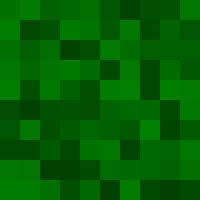
\includegraphics[width=0.25\textwidth]{ps0/sprite.jpg}
    \caption{Sprite Image}
    \label{fig:mesh1}
\end{figure}

\subsection{What I learned :}\label{sec:ps0:learn}

I learned to use SFML for the first time and also how to add events and manipulate them in the SFML field.
Overall, It was fun to do this assignment, as everything for me in this assignment was new an amazing.


\subsection{Acknowledgements:}
\begin{itemize}
    \item \url{https://www.sfml-dev.org/tutorials/2.5/}
    \item \url{https://youtu.be/axIgxBQVBg0}
\end{itemize}


\subsection{Codebase}\label{sec:ps0:code}

\colorbox{pink}{\textbf{main.cpp:}} \newline \textbf{The main file where the code runs and provides the valid output as shown in figure 2.}
\lstinputlisting{ps0/main.cpp}


\subsection{Output:}\label{sec:ps0:output}
\begin{figure}[h]
    \centering
    \includegraphics[width=0.5\textwidth]{ps0/Screenshot.png}
    \caption{Output of PS0 Assignment}
    \label{fig:ps0}
\end{figure}
